\section{Transformations and Compositions}\label{sec:Transformations}

\subsection{Tranformations}
\dfont{Transformations} are operations we can apply to a function in order to obtain a \ifont{new} function.
The most common transformations include translations, stretches and reflections.
We summarize these below.

\begin{center}
\framebox{
$\begin{array}{ccccl}
\mbox{\underline{Function}}&\qquad&\mbox{\underline{Conditions}}&\qquad&\mbox{\underline{How to graph $F(x)$ given the graph of $f(x)$}}\\
F(x)=f(x)+c&\qquad&c>0&\qquad&\mbox{Shift $f(x)$ upwards by $c$ units}\\
F(x)=f(x)-c&\qquad&c>0&\qquad&\mbox{Shift $f(x)$ downwards by $c$ units}\\
F(x)=f(x+c)&\qquad&c>0&\qquad&\mbox{Shift $f(x)$ to the left by $c$ units}\\
F(x)=f(x-c)&\qquad&c>0&\qquad&\mbox{Shift $f(x)$ to the right by $c$ units}\\
\hline
F(x)=-f(x)&\qquad&~&\qquad&\mbox{Reflect $f(x)$ about the $x$-axis}\\
F(x)=f(-x)&\qquad&~&\qquad&\mbox{Reflect $f(x)$ about the $y$-axis}\\
\hline
F(x)=|f(x)|&\qquad&~&\qquad&\mbox{Take the part of the graph of $f(x)$ that lies}\\
~&\qquad&~&\qquad&\mbox{below the $x$-axis and reflect it about the $x$-axis}\\
\end{array}$}
\end{center}

For horizontal and vertical stretches, different resources use different terminology and notation. 
Use the one you are most comfortable with!
Below, both $a,b$ are positive numbers. Note that we only use the term \ifont{stretch} in this case:

\begin{center}
\framebox{
$\begin{array}{ccccl}
\mbox{\underline{Function}}&\qquad&\mbox{\underline{Conditions}}&\qquad&\mbox{\underline{How to graph $F(x)$ given the graph of $f(x)$}}\\
F(x)=af(x)&\qquad&a>0&\qquad&\mbox{Stretch $f(x)$ vertically by a factor of $a$}\\
F(x)=f(bx)&\qquad&b>0&\qquad&\mbox{Stretch $f(x)$ horizontally by a factor of $1/b$}\\
\end{array}$}
\end{center}

In the next case, we use both the terms \ifont{stretch} and \ifont{shrink}.
We also split up vertical stretches into two cases ($0<a<1$ and $a>1$), and split up horizontal stretches into two cases ($0<b<1$ and $b>1$).
Note that having $0<a<1$ is the same as having $1/c$ with $c>1$.
Also note that \ifont{stretching by a factor of $1/c$} is the same as \ifont{shrinking by a factor $c$}.

\begin{center}
\framebox{ 
$\begin{array}{ccccl}
\mbox{\underline{Function}}&\qquad&\mbox{\underline{Conditions}}&\qquad&\mbox{\underline{How to graph $F(x)$ given the graph of $f(x)$}}\\
F(x)=cf(x)&\qquad&c>1&\qquad&\mbox{Stretch $f(x)$ vertically by a factor of $c$}\\
F(x)=(1/c)f(x)&\qquad&c>1&\qquad&\mbox{Shrink $f(x)$ vertically by a factor of $c$}\\
F(x)=f(cx)&\qquad&c>1&\qquad&\mbox{Shrink $f(x)$ horizontally by a factor of $c$}\\
F(x)=f(x/c)&\qquad&c>1&\qquad&\mbox{Stretch $f(x)$ horizontally by a factor of $c$}\\
\end{array}$}
\end{center}

Some resources keep the condition $0<c<1$ rather than using $1/c$.
This is illustrated in the next table.

\begin{center}
\framebox{
$\begin{array}{ccccl}
\mbox{\underline{Function}}&\qquad&\mbox{\underline{Conditions}}&\qquad&\mbox{\underline{How to graph $F(x)$ given the graph of $f(x)$}}\\
F(x)=df(x)&\qquad&d>1&\qquad&\mbox{Stretch $f(x)$ vertically by a factor of $d$}\\
F(x)=df(x)&\qquad&0<d<1&\qquad&\mbox{Shrink $f(x)$ vertically by a factor of $1/d$}\\
F(x)=f(dx)&\qquad&d>1&\qquad&\mbox{Shrink $f(x)$ horizontally by a factor of $d$}\\
F(x)=f(dx)&\qquad&0<d<1&\qquad&\mbox{Stretch $f(x)$ horizontally by a factor of $1/d$}\\
\end{array}$}
\end{center}

\begin{example}{Transformations and Graph Sketching}{TransformationsGraphSketching}
In this example we will use appropriate transformations to sketch the graph of the function $y=|\sqrt{x+2}-1|-1$.
\end{example}
\begin{solution} 
We start with the graph of a function we know how to sketch, in particular, $y=\sqrt{x}$:
To obtain the graph of the function $y=\sqrt{x+2}$ from the graph $y=\sqrt{x}$, we must shift $y=\sqrt{x}$ to the left by $2$ units.
To obtain the graph of the function $y=\sqrt{x+2}-1$ from the graph $y=\sqrt{x+2}$, we must shift $y=\sqrt{x+2}$ downwards by $1$ unit.
$$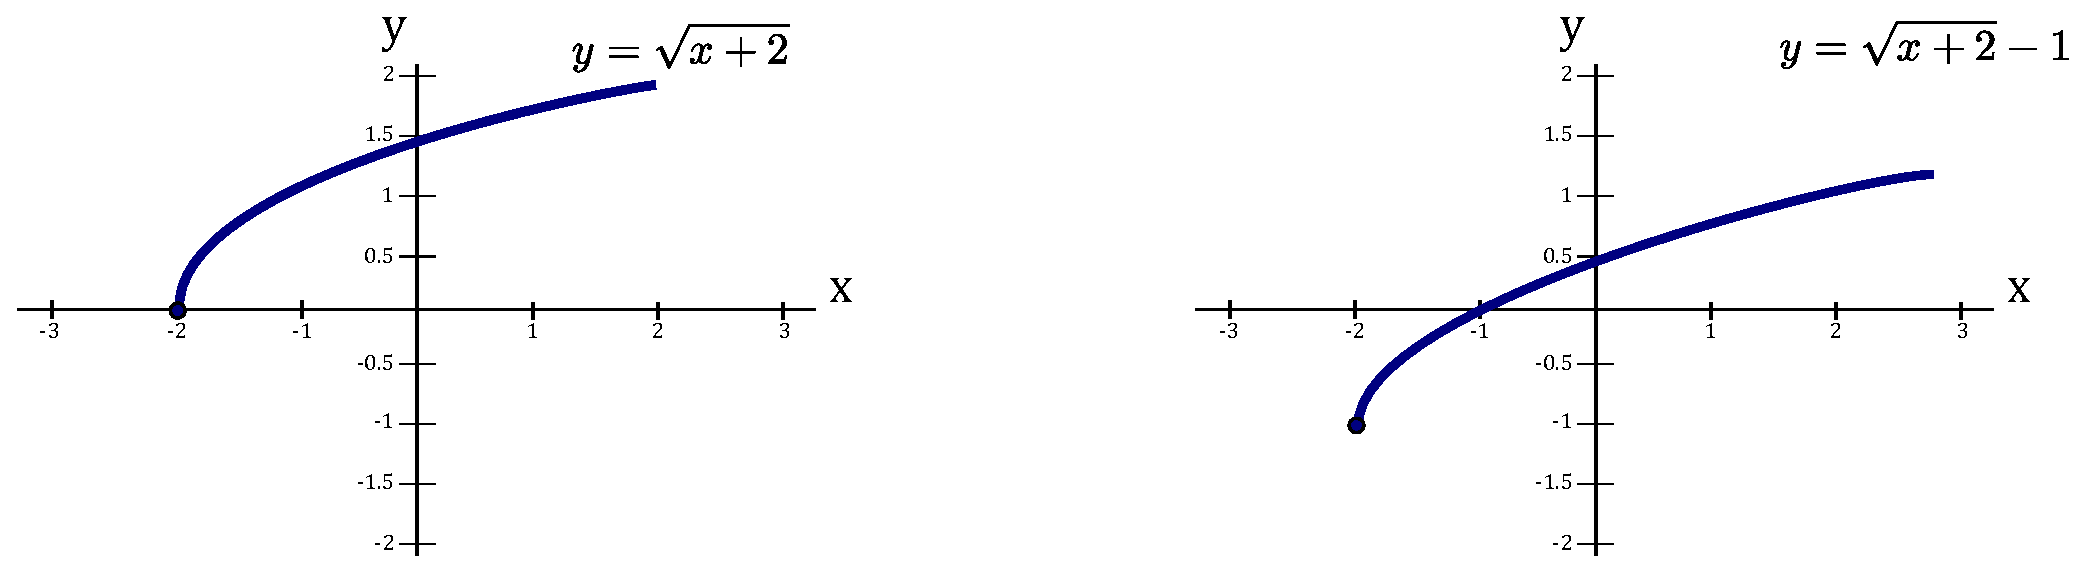
\includegraphics[width=6in]{images/transf1}$$
To obtain the graph of the function $y=|\sqrt{x+2}-1|$ from the graph $y=\sqrt{x+2}-1$, we must take the part of the graph of $y=\sqrt{x+2}-1$ that lies below the $x$-axis and reflect it (upwards) about the $x$-axis.
Finally, to obtain the graph of the function $y=|\sqrt{x+2}-1|-1$ from the graph $y=|\sqrt{x+2}-1|$, we must shift $y=|\sqrt{x+2}-1|$ downwards by $1$ unit:
$$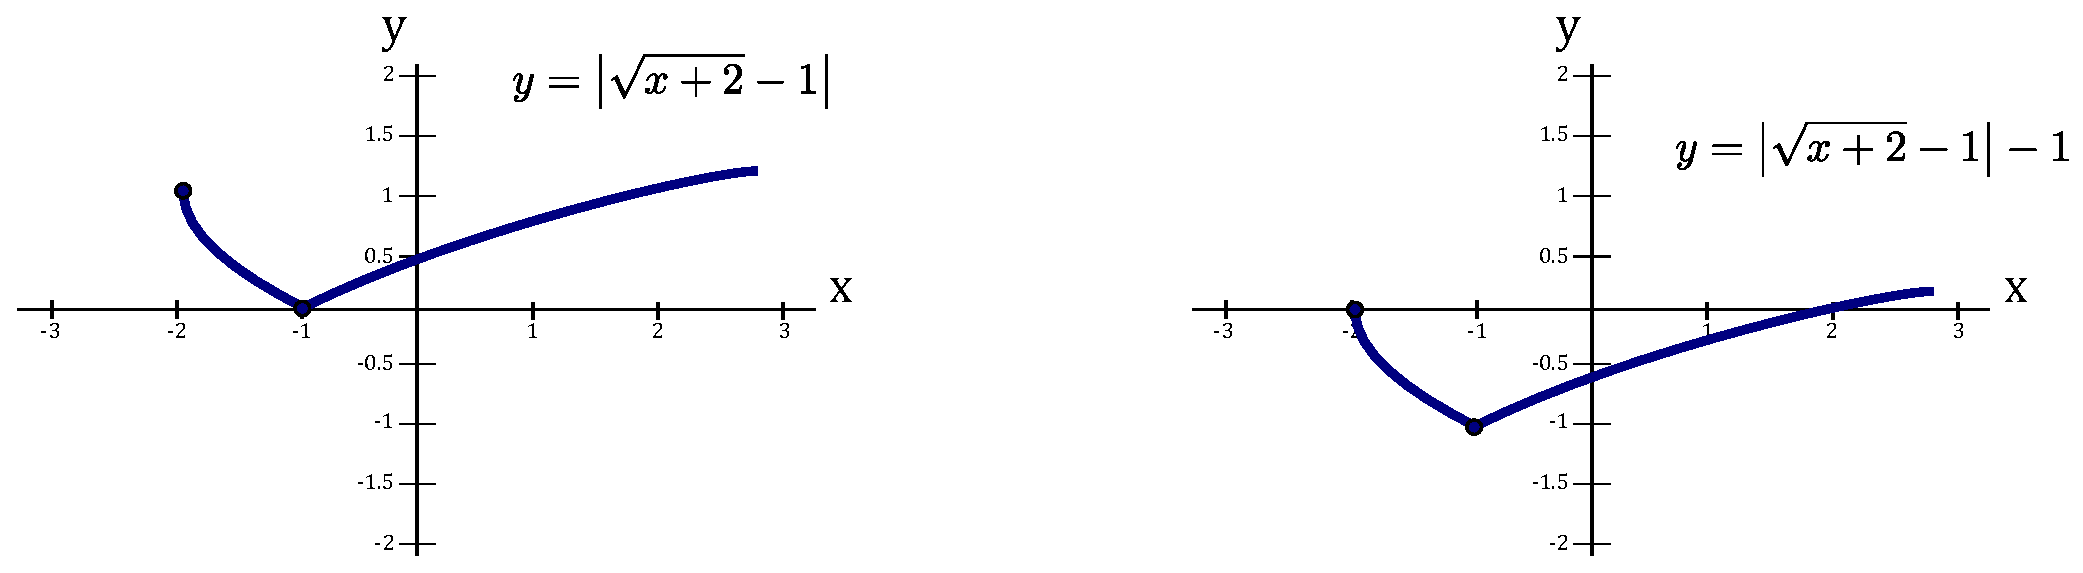
\includegraphics[width=6in]{images/transf2}$$
\end{solution}
\subsection{Combining Two Functions}
Let $f$ and $g$ be two functions.
Then we can form new functions by adding, subtracting, multiplying, or dividing.
These new functions, $f+g$, $f-g$, $fg$ and $f/g$, are defined in the usual way.

\begin{formulabox}[Operations on Functions]
$$(f+g)(x)=f(x)+g(x)\qquad \qquad (f-g)(x)=f(x)-g(x)$$
$$(fg)(x)=f(x)g(x)\qquad \qquad \left(\frac{f}{g}\right)(x)=\frac{f(x)}{g(x)}$$
\end{formulabox}

Suppose $D_f$ is the domain of $f$ and $D_g$ is the domain of $g$.
Then the domains of $f+g$, $f-g$ and $fg$ are the same and are equal to the intersection $D_f\cap D_g$ (that is, everything that is in \ifont{common} to both the domain of $f$ and the domain of $g$).
Since division by zero is \ifont{not allowed}, the domain of $f/g$ is $\{x\in D_f\cap D_g:g(x)\neq 0\}$.

Another way to combine two functions $f$ and $g$ together is a procedure called composition.

\begin{formulabox}[Function Composition]
Given two functions $f$ and $g$, the \ffont{composition} of $f$ and $g$, denoted by $f\circ g$, is defined as:
$$(f\circ g)(x)=f(g(x)).$$
\end{formulabox}

The domain of $f\circ g$ is $\{x\in D_g:g(x)\in D_f\}$, that is, it contains all values $x$ in the domain of $g$ such that $g(x)$ is in the domain of $f$.

\begin{example}{Domain of a Composition}{DomainofaComposition}
Let $f(x)=x^2$ and $g(x)=\sqrt x$.
Find the domain of $f\circ g$.
\end{example}

\begin{solution}
The domain of $f$ is $D_f=\{x\in\R\}$. 
The domain of $g$ is $D_g=\{x\in\R:x\geq 0\}$.
The function $(f\circ g)(x)=f(g(x))$ is:
$$f(g(x))=\left(\sqrt x\right)^2=x.$$
Typically, $h(x)=x$ would have a domain of $\{x\in\R\}$, but since it came from a {\bf composed function}, we must consider $g(x)$ when looking at the domain of $f(g(x))$. 
Thus, the domain of $f\circ g$ is $\{x\in\R:x\geq 0\}$.
\end{solution}

\begin{example}{Combining Two Functions}{CombiningTwoFunctions}
Let $f(x)=x^2+3$ and $g(x)=x-2$.
Find $f+g$, $f-g$, $fg$, $f/g$, $f\circ g$ and $g\circ f$.
Also, determine the domains of these new functions.
\end{example}

\begin{solution} 
For $f+g$ we have:
$$(f+g)(x)=f(x)+g(x)=(x^2+3)+(x-2)=x^2+x+1.$$
For $f-g$ we have:
$$(f-g)(x)=f(x)-g(x)=(x^2+3)-(x-2)=x^2+3-x+2=x^2-x+5.$$
For $fg$ we have:
$$(fg)(x)=f(x)\cdot g(x)=(x^2+3)(x-2)=x^3-2x^2+3x-6.$$
For $f/g$ we have:
$$\left(\frac{f}{g}\right)(x)=\frac{f(x)}{g(x)}=\frac{x^2+3}{x-2}.$$
For $f\circ g$ we have:
$$(f\circ g)(x)=f(g(x))=f(x-2)=(x-2)^2+3=x^2-4x+7.$$
For $g\circ f$ we have:
$$(g\circ f)(x)=g(f(x))=g(x^2+3)=(x^2+3)-2=x^2+1.$$
The domains of $f+g$, $f-g$, $fg$, $f\circ g$ and $g\circ f$ is $\{x\in\mathbb{R}\}$, while the domain of $f/g$ is $\{x\in\mathbb{R}\,:\,x\neq 2\}$.
\end{solution}

As in the above problem, $f\circ g$ and $g\circ f$ are generally different functions.

%%%%%%%%%%%%%%%%%%%%%%%%%%%%%%%%%%%%%%%%%%%%%%%%%%
\Opensolutionfile{solutions}[ex]
\section*{Exercises for \ref{sec:Transformations}}

\begin{enumialphparenastyle}

%%%%%%%%%%
\begin{ex}
Starting with the graph of $\ds y=\sqrt{x}$, the graph of $\ds y=1/x$, and the
graph of $\ds y=\sqrt{1-x^2}$ (the upper unit semicircle), sketch the
graph of each of the following functions:
\begin{multicols}{2}
\begin{enumerate}
	\item	$\ds f(x)=\sqrt{x-2}$
	\item	$\ds f(x)=-1-1/(x+2)$
	\item	$\ds f(x)=4+\sqrt{x+2}$
	\item	$\ds y=f(x)=x/(1-x)$
	\item	$\ds y=f(x)=-\sqrt{-x}$
	\item	$\ds f(x)=2+\sqrt{1-(x-1)^2}$
	\item	$\ds f(x)=-4+\sqrt{-(x-2)}$
	\item	$\ds f(x)=2\sqrt{1-(x/3)^2}$
	\item	$\ds f(x)=1/(x+1)$
	\item	$\ds f(x)=4+2\sqrt{1-(x-5)^2/9}$
	\item	$\ds f(x)=1+1/(x-1)$
	\item	$\ds f(x)=\sqrt{100-25(x-1)^2}+2$
\end{enumerate}
\end{multicols}
\end{ex}

%%%%%%%%%%
\begin{ex}
The graph of $f(x)$ is shown below.
Sketch the graphs of the following functions.
\vadjust{\rightline{%
\vbox to 0pt{\vskip-5pt\beginpicture
\normalgraphs
\setcoordinatesystem units <1truecm,1truecm>
\setplotarea x from 0 to 3.25, y from -1.5 to 2
\axis bottom shiftedto y=0 ticks numbered from 1 to 3 by 1 /
\axis left ticks numbered from -1 to 2 by 1 /
\setquadratic
\plot 
0.000 -1.285 0.054 -0.643 0.108 -0.088 0.162 0.387 0.217 0.788 
0.271 1.120 0.325 1.391 0.379 1.604 0.433 1.766 0.488 1.882 
0.542 1.956 0.596 1.993 0.650 1.998 0.704 1.976 0.758 1.929 
0.812 1.862 0.867 1.779 0.921 1.684 0.975 1.578 1.029 1.467 
1.083 1.351 1.138 1.235 1.192 1.120 1.246 1.008 1.300 0.903 
1.354 0.805 1.408 0.716 1.462 0.637 1.517 0.571 1.571 0.517 
1.625 0.476 1.679 0.450 1.733 0.438 1.788 0.441 1.842 0.458 
1.896 0.490 1.950 0.536 2.004 0.595 2.058 0.666 2.112 0.749 
2.167 0.841 2.221 0.943 2.275 1.051 2.329 1.164 2.383 1.279 
2.438 1.396 2.492 1.510 2.546 1.620 2.600 1.722 2.654 1.813 
2.708 1.890 2.762 1.949 2.817 1.987 2.871 2.000 2.925 1.983 
2.979 1.932 3.033 1.842 3.088 1.710 3.142 1.528 3.196 1.294 
3.250 1.000 /
\endpicture\vskip0pt\vss}\hskip8cm}}
\vspace{1.5in}

\begin{multicols}{2}
\begin{enumerate}
	\item	$\ds y=f(x-1)$
	\item	$\ds y=1+f(x+2)$
	\item	$\ds y=1+2f(x)$
	\item	$\ds y=2f(3x)$
	\item	$\ds y=2f(3(x-2))+1$
	\item	$\ds y=(1/2)f(3x-3)$
	\item	$\ds y=f(1+x/3)+2$
	\item	$\ds y=|f(x)-2|$
\end{enumerate}
\end{multicols}
\end{ex}

%%%%%%%%%%
\begin{ex}
Suppose $f(x) = 3x-9$ and $\ds g(x) = \sqrt{x}$.  What is the
domain of the composition $(g\circ f)(x)$?
\begin{sol}
$\ds \{x\mid x\ge3\}$, $\{x\mid x\ge0\}$
\end{sol}
\end{ex}

\end{enumialphparenastyle}